% Options for packages loaded elsewhere
\PassOptionsToPackage{unicode}{hyperref}
\PassOptionsToPackage{hyphens}{url}
\PassOptionsToPackage{dvipsnames,svgnames,x11names}{xcolor}
%
\documentclass[
  letterpaper,
  DIV=11,
  numbers=noendperiod]{scrartcl}

\usepackage{amsmath,amssymb}
\usepackage{lmodern}
\usepackage{iftex}
\ifPDFTeX
  \usepackage[T1]{fontenc}
  \usepackage[utf8]{inputenc}
  \usepackage{textcomp} % provide euro and other symbols
\else % if luatex or xetex
  \usepackage{unicode-math}
  \defaultfontfeatures{Scale=MatchLowercase}
  \defaultfontfeatures[\rmfamily]{Ligatures=TeX,Scale=1}
\fi
% Use upquote if available, for straight quotes in verbatim environments
\IfFileExists{upquote.sty}{\usepackage{upquote}}{}
\IfFileExists{microtype.sty}{% use microtype if available
  \usepackage[]{microtype}
  \UseMicrotypeSet[protrusion]{basicmath} % disable protrusion for tt fonts
}{}
\makeatletter
\@ifundefined{KOMAClassName}{% if non-KOMA class
  \IfFileExists{parskip.sty}{%
    \usepackage{parskip}
  }{% else
    \setlength{\parindent}{0pt}
    \setlength{\parskip}{6pt plus 2pt minus 1pt}}
}{% if KOMA class
  \KOMAoptions{parskip=half}}
\makeatother
\usepackage{xcolor}
\setlength{\emergencystretch}{3em} % prevent overfull lines
\setcounter{secnumdepth}{-\maxdimen} % remove section numbering
% Make \paragraph and \subparagraph free-standing
\ifx\paragraph\undefined\else
  \let\oldparagraph\paragraph
  \renewcommand{\paragraph}[1]{\oldparagraph{#1}\mbox{}}
\fi
\ifx\subparagraph\undefined\else
  \let\oldsubparagraph\subparagraph
  \renewcommand{\subparagraph}[1]{\oldsubparagraph{#1}\mbox{}}
\fi

\usepackage{color}
\usepackage{fancyvrb}
\newcommand{\VerbBar}{|}
\newcommand{\VERB}{\Verb[commandchars=\\\{\}]}
\DefineVerbatimEnvironment{Highlighting}{Verbatim}{commandchars=\\\{\}}
% Add ',fontsize=\small' for more characters per line
\usepackage{framed}
\definecolor{shadecolor}{RGB}{241,243,245}
\newenvironment{Shaded}{\begin{snugshade}}{\end{snugshade}}
\newcommand{\AlertTok}[1]{\textcolor[rgb]{0.68,0.00,0.00}{#1}}
\newcommand{\AnnotationTok}[1]{\textcolor[rgb]{0.37,0.37,0.37}{#1}}
\newcommand{\AttributeTok}[1]{\textcolor[rgb]{0.40,0.45,0.13}{#1}}
\newcommand{\BaseNTok}[1]{\textcolor[rgb]{0.68,0.00,0.00}{#1}}
\newcommand{\BuiltInTok}[1]{\textcolor[rgb]{0.00,0.23,0.31}{#1}}
\newcommand{\CharTok}[1]{\textcolor[rgb]{0.13,0.47,0.30}{#1}}
\newcommand{\CommentTok}[1]{\textcolor[rgb]{0.37,0.37,0.37}{#1}}
\newcommand{\CommentVarTok}[1]{\textcolor[rgb]{0.37,0.37,0.37}{\textit{#1}}}
\newcommand{\ConstantTok}[1]{\textcolor[rgb]{0.56,0.35,0.01}{#1}}
\newcommand{\ControlFlowTok}[1]{\textcolor[rgb]{0.00,0.23,0.31}{#1}}
\newcommand{\DataTypeTok}[1]{\textcolor[rgb]{0.68,0.00,0.00}{#1}}
\newcommand{\DecValTok}[1]{\textcolor[rgb]{0.68,0.00,0.00}{#1}}
\newcommand{\DocumentationTok}[1]{\textcolor[rgb]{0.37,0.37,0.37}{\textit{#1}}}
\newcommand{\ErrorTok}[1]{\textcolor[rgb]{0.68,0.00,0.00}{#1}}
\newcommand{\ExtensionTok}[1]{\textcolor[rgb]{0.00,0.23,0.31}{#1}}
\newcommand{\FloatTok}[1]{\textcolor[rgb]{0.68,0.00,0.00}{#1}}
\newcommand{\FunctionTok}[1]{\textcolor[rgb]{0.28,0.35,0.67}{#1}}
\newcommand{\ImportTok}[1]{\textcolor[rgb]{0.00,0.46,0.62}{#1}}
\newcommand{\InformationTok}[1]{\textcolor[rgb]{0.37,0.37,0.37}{#1}}
\newcommand{\KeywordTok}[1]{\textcolor[rgb]{0.00,0.23,0.31}{#1}}
\newcommand{\NormalTok}[1]{\textcolor[rgb]{0.00,0.23,0.31}{#1}}
\newcommand{\OperatorTok}[1]{\textcolor[rgb]{0.37,0.37,0.37}{#1}}
\newcommand{\OtherTok}[1]{\textcolor[rgb]{0.00,0.23,0.31}{#1}}
\newcommand{\PreprocessorTok}[1]{\textcolor[rgb]{0.68,0.00,0.00}{#1}}
\newcommand{\RegionMarkerTok}[1]{\textcolor[rgb]{0.00,0.23,0.31}{#1}}
\newcommand{\SpecialCharTok}[1]{\textcolor[rgb]{0.37,0.37,0.37}{#1}}
\newcommand{\SpecialStringTok}[1]{\textcolor[rgb]{0.13,0.47,0.30}{#1}}
\newcommand{\StringTok}[1]{\textcolor[rgb]{0.13,0.47,0.30}{#1}}
\newcommand{\VariableTok}[1]{\textcolor[rgb]{0.07,0.07,0.07}{#1}}
\newcommand{\VerbatimStringTok}[1]{\textcolor[rgb]{0.13,0.47,0.30}{#1}}
\newcommand{\WarningTok}[1]{\textcolor[rgb]{0.37,0.37,0.37}{\textit{#1}}}

\providecommand{\tightlist}{%
  \setlength{\itemsep}{0pt}\setlength{\parskip}{0pt}}\usepackage{longtable,booktabs,array}
\usepackage{calc} % for calculating minipage widths
% Correct order of tables after \paragraph or \subparagraph
\usepackage{etoolbox}
\makeatletter
\patchcmd\longtable{\par}{\if@noskipsec\mbox{}\fi\par}{}{}
\makeatother
% Allow footnotes in longtable head/foot
\IfFileExists{footnotehyper.sty}{\usepackage{footnotehyper}}{\usepackage{footnote}}
\makesavenoteenv{longtable}
\usepackage{graphicx}
\makeatletter
\def\maxwidth{\ifdim\Gin@nat@width>\linewidth\linewidth\else\Gin@nat@width\fi}
\def\maxheight{\ifdim\Gin@nat@height>\textheight\textheight\else\Gin@nat@height\fi}
\makeatother
% Scale images if necessary, so that they will not overflow the page
% margins by default, and it is still possible to overwrite the defaults
% using explicit options in \includegraphics[width, height, ...]{}
\setkeys{Gin}{width=\maxwidth,height=\maxheight,keepaspectratio}
% Set default figure placement to htbp
\makeatletter
\def\fps@figure{htbp}
\makeatother

\KOMAoption{captions}{tableheading}
\makeatletter
\makeatother
\makeatletter
\makeatother
\makeatletter
\@ifpackageloaded{caption}{}{\usepackage{caption}}
\AtBeginDocument{%
\ifdefined\contentsname
  \renewcommand*\contentsname{Table of contents}
\else
  \newcommand\contentsname{Table of contents}
\fi
\ifdefined\listfigurename
  \renewcommand*\listfigurename{List of Figures}
\else
  \newcommand\listfigurename{List of Figures}
\fi
\ifdefined\listtablename
  \renewcommand*\listtablename{List of Tables}
\else
  \newcommand\listtablename{List of Tables}
\fi
\ifdefined\figurename
  \renewcommand*\figurename{Figure}
\else
  \newcommand\figurename{Figure}
\fi
\ifdefined\tablename
  \renewcommand*\tablename{Table}
\else
  \newcommand\tablename{Table}
\fi
}
\@ifpackageloaded{float}{}{\usepackage{float}}
\floatstyle{ruled}
\@ifundefined{c@chapter}{\newfloat{codelisting}{h}{lop}}{\newfloat{codelisting}{h}{lop}[chapter]}
\floatname{codelisting}{Listing}
\newcommand*\listoflistings{\listof{codelisting}{List of Listings}}
\makeatother
\makeatletter
\@ifpackageloaded{caption}{}{\usepackage{caption}}
\@ifpackageloaded{subcaption}{}{\usepackage{subcaption}}
\makeatother
\makeatletter
\@ifpackageloaded{tcolorbox}{}{\usepackage[many]{tcolorbox}}
\makeatother
\makeatletter
\@ifundefined{shadecolor}{\definecolor{shadecolor}{rgb}{.97, .97, .97}}
\makeatother
\makeatletter
\makeatother
\ifLuaTeX
  \usepackage{selnolig}  % disable illegal ligatures
\fi
\IfFileExists{bookmark.sty}{\usepackage{bookmark}}{\usepackage{hyperref}}
\IfFileExists{xurl.sty}{\usepackage{xurl}}{} % add URL line breaks if available
\urlstyle{same} % disable monospaced font for URLs
\hypersetup{
  pdftitle={Introduction to Mapping in R},
  colorlinks=true,
  linkcolor={blue},
  filecolor={Maroon},
  citecolor={Blue},
  urlcolor={Blue},
  pdfcreator={LaTeX via pandoc}}

\title{Introduction to Mapping in R}
\author{}
\date{}

\begin{document}
\maketitle
\ifdefined\Shaded\renewenvironment{Shaded}{\begin{tcolorbox}[boxrule=0pt, breakable, enhanced, frame hidden, borderline west={3pt}{0pt}{shadecolor}, interior hidden, sharp corners]}{\end{tcolorbox}}\fi

\hypertarget{resources-used}{%
\subsection{Resources used:}\label{resources-used}}

https://r-spatial.org/r/2018/10/25/ggplot2-sf.html
https://r-spatial.github.io/sf/articles/sf1.html
https://r-spatial.github.io/sf/articles/sf2.html\#using-st\_read
https://r-spatial.github.io/sf/articles/sf3.html
https://r-spatial.github.io/sf/articles/sf4.html
https://r-spatial.github.io/sf/articles/sf6.html
https://r-spatial.github.io/sf/articles/sf7.html
https://github.com/BenMarmont/AARES-R-Workshop/blob/main/\_AARES/introduction\%20to\%20R\%20for\%20economists.R

\hypertarget{r-and-mapping}{%
\subsection{R and Mapping}\label{r-and-mapping}}

Current solutions for creating maps usually involves GIS software, such
as ArcGIS, QGIS, eSpatial, etc., which allow to visually prepare a map,
in the same approach as one would prepare a poster or a document layout.
On the other hand, R, a free and open-source software development
environment (IDE) that is used for computing statistical data and
graphic in a programmable language, has developed advanced spatial
capabilities over the years, and can be used to draw maps
programmatically.

R is a powerful and flexible tool. R can be used from calculating data
sets to creating graphs and maps with the same data set. R is also free,
which makes it easily accessible to anyone. Some other advantages of
using R is that it has an interactive language, data structures,
graphics availability, a developed community, and the advantage of
adding more functionalities through an entire ecosystem of packages. R
is a scriptable language that allows the user to write out a code in
which it will execute the commands specified.

Using R to create maps brings these benefits to mapping. Elements of a
map can be added or removed with ease --- R code can be tweaked to make
major enhancements with a stroke of a key. It is also easy to reproduce
the same maps for different data sets. It is important to be able to
script the elements of a map, so that it can be re-used and interpreted
by any user. In essence, comparing typical GIS software and R for
drawing maps is similar to comparing word processing software
(e.g.~Microsoft Office or LibreOffice) and a programmatic typesetting
system such as LaTeX, in that typical GIS software implement a WYSIWIG
approach (``What You See Is What You Get''), while R implements a
WYSIWYM approach (``What You See Is What You Mean'').

The package \texttt{ggplot2} implements the grammar of graphics in R, as
a way to create code that make sense to the user: The grammar of
graphics is a term used to breaks up graphs into semantic components,
such as geometries and layers. Practically speaking, it allows (and
forces!) the user to focus on graph elements at a higher level of
abstraction, and how the data must be structured to achieve the expected
outcome. While \texttt{ggplot2} is becoming the de facto standard for R
graphs, it does not handle spatial data specifically. The current
state-of-the-art of spatial objects in R relies on \texttt{Spatial}
classes defined in the package
\href{https://cran.r-project.org/package=sp}{\texttt{sp}}, but the new
package \href{https://cran.r-project.org/package=sf}{\texttt{sf}} has
recently implemented the ``simple feature'' standard, and is steadily
taking over \texttt{sp}. Recently, the package \texttt{ggplot2} has
allowed the use of simple features from the package \texttt{sf} as
layers in a
graph\textsuperscript{\href{https://r-spatial.org/r/2018/10/25/ggplot2-sf.html\#fn:1}{1}}.
The combination of \texttt{ggplot2} and \texttt{sf} therefore enables to
programmatically create maps, using the grammar of graphics, just as
informative or visually appealing as traditional GIS software.

\hypertarget{mapping-with-ggplot}{%
\subsection{Mapping with ggplot}\label{mapping-with-ggplot}}

First, lets make some plots created with our old faithful, ggplot. THe
data used for these plots comes with the tidyverse!

\begin{Shaded}
\begin{Highlighting}[]
\CommentTok{\#\textquotesingle{}label: ggplot maps}
\FunctionTok{library}\NormalTok{(tidyverse)}
\end{Highlighting}
\end{Shaded}

\begin{verbatim}
-- Attaching core tidyverse packages ------------------------ tidyverse 2.0.0 --
v dplyr     1.1.2     v readr     2.1.4
v forcats   1.0.0     v stringr   1.5.0
v ggplot2   3.4.2     v tibble    3.2.1
v lubridate 1.9.2     v tidyr     1.3.0
v purrr     1.0.1     
-- Conflicts ------------------------------------------ tidyverse_conflicts() --
x dplyr::filter() masks stats::filter()
x dplyr::lag()    masks stats::lag()
i Use the conflicted package (<http://conflicted.r-lib.org/>) to force all conflicts to become errors
\end{verbatim}

\begin{Shaded}
\begin{Highlighting}[]
\CommentTok{\# ggplot maps are static}

\CommentTok{\# World map}

\FunctionTok{map\_data}\NormalTok{(}\StringTok{"world"}\NormalTok{) }\SpecialCharTok{|\textgreater{}} 
  \FunctionTok{ggplot}\NormalTok{(}\FunctionTok{aes}\NormalTok{(long, lat, }\AttributeTok{group =}\NormalTok{ group)) }\SpecialCharTok{+} 
  \FunctionTok{geom\_polygon}\NormalTok{()}
\end{Highlighting}
\end{Shaded}

\begin{figure}[H]

{\centering 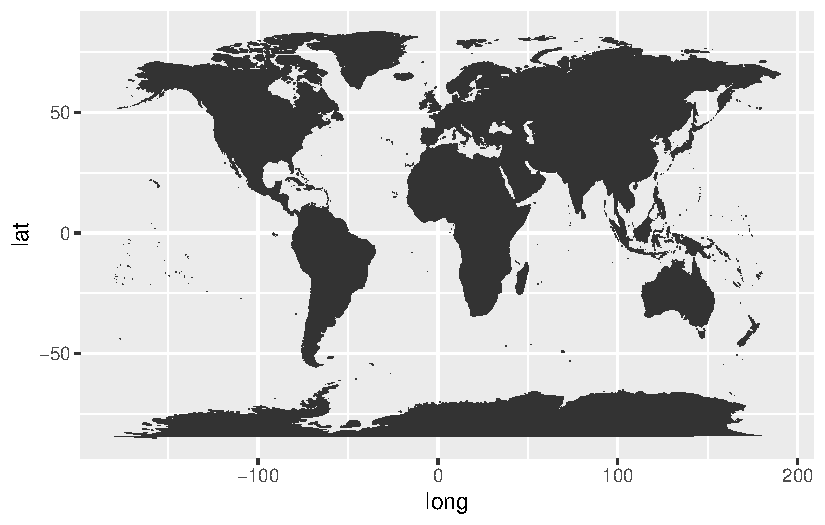
\includegraphics{Introduction-to-mapping_files/figure-pdf/unnamed-chunk-1-1.pdf}

}

\end{figure}

\begin{Shaded}
\begin{Highlighting}[]
\CommentTok{\# New Zealand map}

\NormalTok{world\_map }\OtherTok{\textless{}{-}} \FunctionTok{map\_data}\NormalTok{(}\StringTok{"world"}\NormalTok{, }\AttributeTok{region =} \StringTok{"New Zealand"}\NormalTok{)}

\FunctionTok{ggplot}\NormalTok{(world\_map, }\FunctionTok{aes}\NormalTok{(long, lat, }\AttributeTok{group =}\NormalTok{ group)) }\SpecialCharTok{+}
  \FunctionTok{geom\_polygon}\NormalTok{()}
\end{Highlighting}
\end{Shaded}

\begin{figure}[H]

{\centering 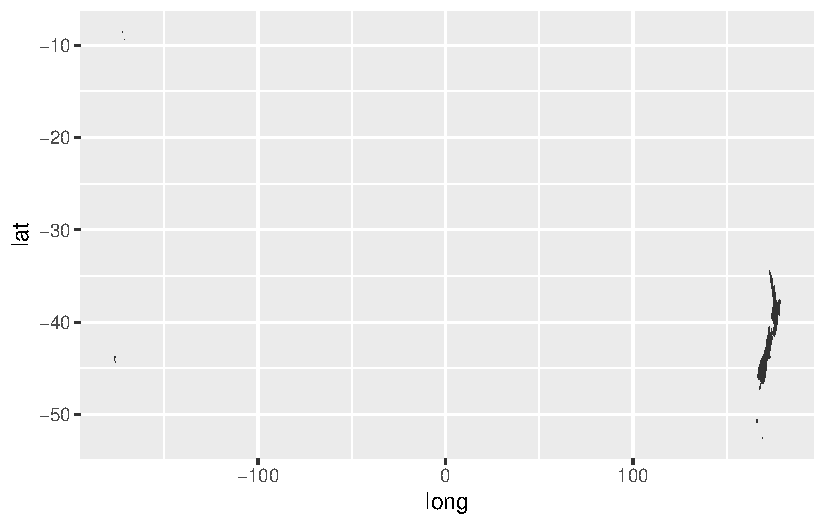
\includegraphics{Introduction-to-mapping_files/figure-pdf/unnamed-chunk-1-2.pdf}

}

\end{figure}

Although, we can make them more `map-like' really quickly with a
function we will look into more shortly.

\begin{Shaded}
\begin{Highlighting}[]
\CommentTok{\#|label: improving ggplot maps}

\FunctionTok{library}\NormalTok{(sf)}
\end{Highlighting}
\end{Shaded}

\begin{verbatim}
Linking to GEOS 3.11.2, GDAL 3.6.2, PROJ 9.2.0; sf_use_s2() is TRUE
\end{verbatim}

\begin{Shaded}
\begin{Highlighting}[]
\CommentTok{\# fixing display using coord\_sf from the sf package}
\FunctionTok{ggplot}\NormalTok{(world\_map, }\FunctionTok{aes}\NormalTok{(long, lat, }\AttributeTok{group =}\NormalTok{ group)) }\SpecialCharTok{+}
  \FunctionTok{geom\_polygon}\NormalTok{() }\SpecialCharTok{+}
  \FunctionTok{coord\_sf}\NormalTok{()}
\end{Highlighting}
\end{Shaded}

\begin{figure}[H]

{\centering 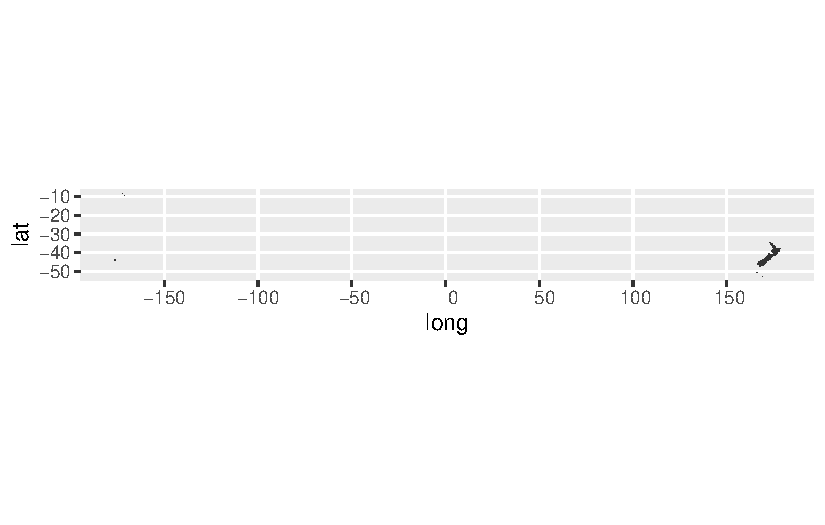
\includegraphics{Introduction-to-mapping_files/figure-pdf/unnamed-chunk-2-1.pdf}

}

\end{figure}

\begin{Shaded}
\begin{Highlighting}[]
\FunctionTok{map\_data}\NormalTok{(}\StringTok{"world"}\NormalTok{) }\SpecialCharTok{|\textgreater{}} 
  \FunctionTok{ggplot}\NormalTok{(}\FunctionTok{aes}\NormalTok{(long, lat, }\AttributeTok{group =}\NormalTok{ group)) }\SpecialCharTok{+} 
  \FunctionTok{geom\_polygon}\NormalTok{() }\SpecialCharTok{+}
  \FunctionTok{coord\_sf}\NormalTok{()}
\end{Highlighting}
\end{Shaded}

\begin{figure}[H]

{\centering 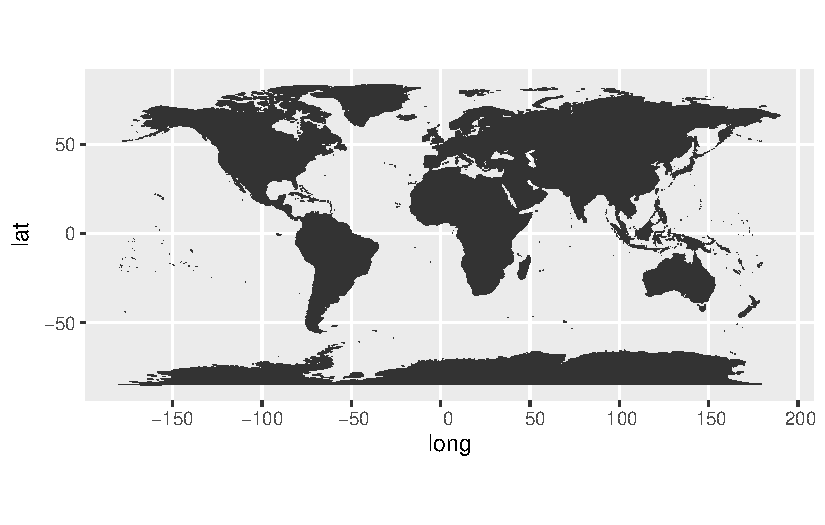
\includegraphics{Introduction-to-mapping_files/figure-pdf/unnamed-chunk-2-2.pdf}

}

\end{figure}

\hypertarget{getting-started}{%
\subsection{Getting started}\label{getting-started}}

Many R packages are available from
\href{https://cran.r-project.org/}{CRAN}, the Comprehensive R Archive
Network, which is the primary repository of R packages. The full list of
packages necessary for this series of tutorials can be installed with:

\begin{Shaded}
\begin{Highlighting}[]
\FunctionTok{install.packages}\NormalTok{(}\FunctionTok{c}\NormalTok{(}\StringTok{"cowplot"}\NormalTok{, }\StringTok{"googleway"}\NormalTok{, }\StringTok{"ggplot2"}\NormalTok{, }\StringTok{"ggrepel"}\NormalTok{,  }\StringTok{"ggspatial"}\NormalTok{, }\StringTok{"libwgeom"}\NormalTok{, }\StringTok{"sf"}\NormalTok{, }\StringTok{"rnaturalearth"}\NormalTok{, }\StringTok{"rnaturalearthdata"}\NormalTok{)) }

                 
\FunctionTok{install.packages}\NormalTok{(}\StringTok{"cowplot"}\NormalTok{)}
\FunctionTok{install.packages}\NormalTok{(}\StringTok{"googleway"}\NormalTok{)}
\FunctionTok{install.packages}\NormalTok{(}\StringTok{"ggrepel"}\NormalTok{)}
\FunctionTok{install.packages}\NormalTok{(}\StringTok{"ggspatial"}\NormalTok{)}
\FunctionTok{install.packages}\NormalTok{(}\StringTok{"libwgeom"}\NormalTok{)}
\FunctionTok{install.packages}\NormalTok{(}\StringTok{"sf"}\NormalTok{)}
\FunctionTok{install.packages}\NormalTok{(}\StringTok{"rnaturalearth"}\NormalTok{)}
\FunctionTok{install.packages}\NormalTok{(}\StringTok{"rnaturalearthdata"}\NormalTok{)                 }
\end{Highlighting}
\end{Shaded}

We start by loading the basic packages necessary for all maps,
i.e.~\texttt{ggplot2} and \texttt{sf}. We also suggest to use the
classic dark-on-light theme for \texttt{ggplot2} (\texttt{theme\_bw}),
which is appropriate for maps:

\begin{Shaded}
\begin{Highlighting}[]
\CommentTok{\#|label: load packages}
\FunctionTok{library}\NormalTok{(ggplot2)}
\FunctionTok{library}\NormalTok{(ggthemes)}
\FunctionTok{library}\NormalTok{(sf) }
\end{Highlighting}
\end{Shaded}

The package \texttt{rnaturalearth} provides a map of countries of the
entire world. Use \texttt{ne\_countries} to pull country data and choose
the scale (\texttt{rnaturalearthhires} is necessary for
\texttt{scale\ =\ "large"}). The function can return \texttt{sp} classes
(default) or directly \texttt{sf} classes, as defined in the argument
\texttt{returnclass}:

Note that sf is preferred and sp is deprecated.

\begin{Shaded}
\begin{Highlighting}[]
\CommentTok{\#|label: settomg up earth data}

\FunctionTok{library}\NormalTok{(}\StringTok{"rnaturalearth"}\NormalTok{) }
\end{Highlighting}
\end{Shaded}

\begin{verbatim}
The legacy packages maptools, rgdal, and rgeos, underpinning this package
will retire shortly. Please refer to R-spatial evolution reports on
https://r-spatial.org/r/2023/05/15/evolution4.html for details.
This package is now running under evolution status 0 
\end{verbatim}

\begin{verbatim}
Support for Spatial objects (`sp`) will be deprecated in {rnaturalearth} and will be removed in a future release of the package. Please use `sf` objects with {rnaturalearth}. For example: `ne_download(returnclass = 'sf')`
\end{verbatim}

\begin{Shaded}
\begin{Highlighting}[]
\FunctionTok{library}\NormalTok{(}\StringTok{"rnaturalearthdata"}\NormalTok{)  }
\end{Highlighting}
\end{Shaded}

\begin{verbatim}

Attaching package: 'rnaturalearthdata'
\end{verbatim}

\begin{verbatim}
The following object is masked from 'package:rnaturalearth':

    countries110
\end{verbatim}

\begin{Shaded}
\begin{Highlighting}[]
\NormalTok{world }\OtherTok{\textless{}{-}} \FunctionTok{ne\_countries}\NormalTok{(}\AttributeTok{scale =} \StringTok{"medium"}\NormalTok{, }\AttributeTok{returnclass =} \StringTok{"sf"}\NormalTok{) }
\NormalTok{nz }\OtherTok{\textless{}{-}} \FunctionTok{ne\_countries}\NormalTok{(}\AttributeTok{country =} \StringTok{"New Zealand"}\NormalTok{, }\AttributeTok{scale =} \StringTok{"medium"}\NormalTok{, }\AttributeTok{returnclass =} \StringTok{"sf"}\NormalTok{)}

\FunctionTok{class}\NormalTok{(world)  }\DocumentationTok{\#\# [1] "sf"   \#\# [1] "data.frame" }
\end{Highlighting}
\end{Shaded}

\begin{verbatim}
[1] "sf"         "data.frame"
\end{verbatim}

\begin{Shaded}
\begin{Highlighting}[]
\FunctionTok{class}\NormalTok{(nz)}
\end{Highlighting}
\end{Shaded}

\begin{verbatim}
[1] "sf"         "data.frame"
\end{verbatim}

\hypertarget{general-concepts-illustrated-with-the-world-map}{%
\section{General concepts illustrated with the world
map}\label{general-concepts-illustrated-with-the-world-map}}

\hypertarget{data-and-basic-plot-ggplot-and-geom_sf}{%
\subsection{\texorpdfstring{Data and basic plot (\texttt{ggplot} and
\texttt{geom\_sf})}{Data and basic plot (ggplot and geom\_sf)}}\label{data-and-basic-plot-ggplot-and-geom_sf}}

First, let us start with creating a base map of the world using
\texttt{ggplot2}. This base map will then be extended with different map
elements, as well as zoomed in to an area of interest. We can check that
the world map was properly retrieved and converted into an \texttt{sf}
object, and plot it with \texttt{ggplot2}:

\begin{Shaded}
\begin{Highlighting}[]
\CommentTok{\#|label: basic ggplot sf map}
\FunctionTok{ggplot}\NormalTok{(}\AttributeTok{data =}\NormalTok{ world) }\SpecialCharTok{+}     \CommentTok{\# this data is coming from the natural earth data}
  \FunctionTok{geom\_sf}\NormalTok{()}
\end{Highlighting}
\end{Shaded}

\begin{figure}[H]

{\centering 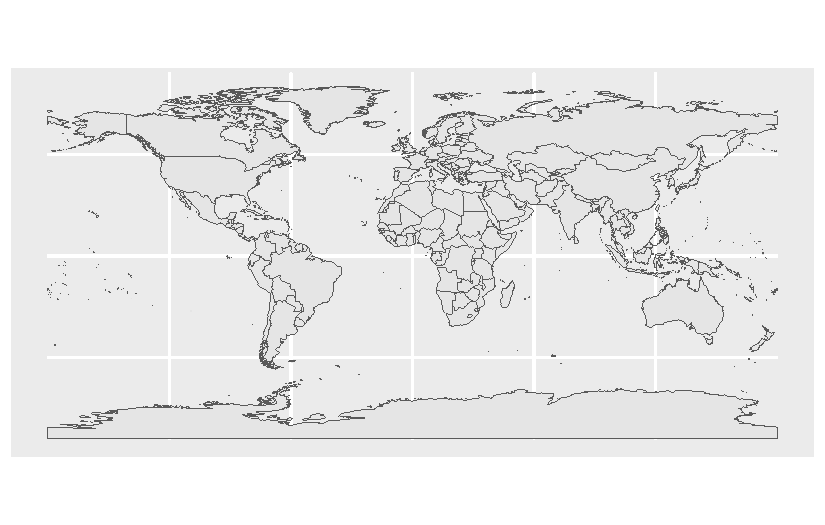
\includegraphics{Introduction-to-mapping_files/figure-pdf/unnamed-chunk-6-1.pdf}

}

\end{figure}

\begin{Shaded}
\begin{Highlighting}[]
\FunctionTok{ggplot}\NormalTok{(}\AttributeTok{data =}\NormalTok{ nz) }\SpecialCharTok{+}     \CommentTok{\# this data is coming from the natural earth data}
  \FunctionTok{geom\_sf}\NormalTok{()}
\end{Highlighting}
\end{Shaded}

\begin{figure}[H]

{\centering 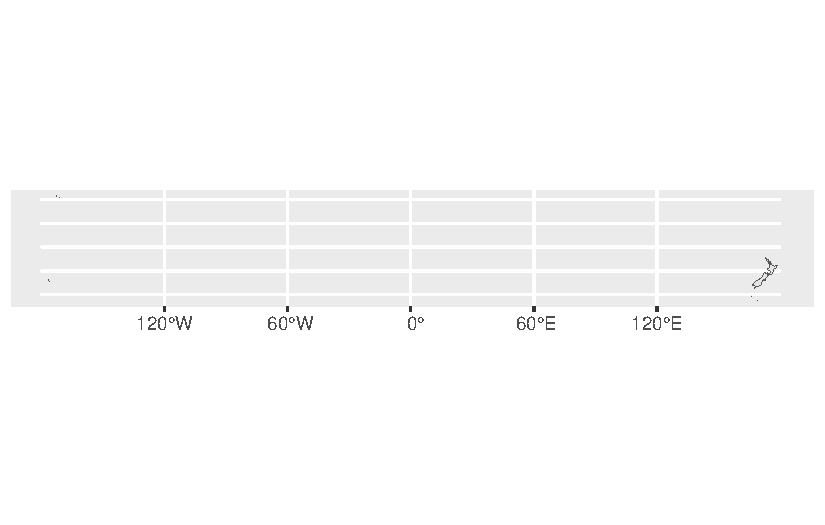
\includegraphics{Introduction-to-mapping_files/figure-pdf/unnamed-chunk-6-2.pdf}

}

\end{figure}

This call nicely introduces the structure of a \texttt{ggplot} call: The
first part \texttt{ggplot(data\ =\ world)} initiates the \texttt{ggplot}
graph, and indicates that the main data is stored in the \texttt{world}
object. The line ends up with a \texttt{+} sign, which indicates that
the call is not complete yet, and each subsequent line correspond to
another layer or scale. In this case, we use the \texttt{geom\_sf}
function, which simply adds a geometry stored in a \texttt{sf} object.
By default, all geometry functions use the main data defined in
\texttt{ggplot()}, but we will see later how to provide additional data.

Note that layers are added one at a time in a \texttt{ggplot} call, so
the order of each layer is very important. All data will have to be in
an \texttt{sf} format to be used by \texttt{ggplot2}; data in other
formats (e.g.~classes from \texttt{sp}) will be manually converted to
\texttt{sf} classes if necessary.

\hypertarget{title-subtitle-and-axis-labels-ggtitle-xlab-ylab}{%
\subsection{\texorpdfstring{Title, subtitle, and axis labels
(\texttt{ggtitle}, \texttt{xlab},
\texttt{ylab})}{Title, subtitle, and axis labels (ggtitle, xlab, ylab)}}\label{title-subtitle-and-axis-labels-ggtitle-xlab-ylab}}

A title and a subtitle can be added to the map using the function
\texttt{ggtitle}, passing any valid character string (e.g.~with
quotation marks) as arguments. Axis names are absent by default on a
map, but can be changed to something more suitable (e.g.~``Longitude''
and ``Latitude''), depending on the map:

Build on your map as you would any other ggplot visualisation!

\begin{Shaded}
\begin{Highlighting}[]
\CommentTok{\#|label: built on ggplot}
\FunctionTok{ggplot}\NormalTok{(}\AttributeTok{data =}\NormalTok{ world) }\SpecialCharTok{+}     
  \FunctionTok{geom\_sf}\NormalTok{() }\SpecialCharTok{+}     
  \FunctionTok{xlab}\NormalTok{(}\StringTok{"Longitude"}\NormalTok{) }\SpecialCharTok{+} 
  \FunctionTok{ylab}\NormalTok{(}\StringTok{"Latitude"}\NormalTok{) }\SpecialCharTok{+}     
  \FunctionTok{ggtitle}\NormalTok{(}\StringTok{"World map"}\NormalTok{) }
\end{Highlighting}
\end{Shaded}

\begin{figure}[H]

{\centering 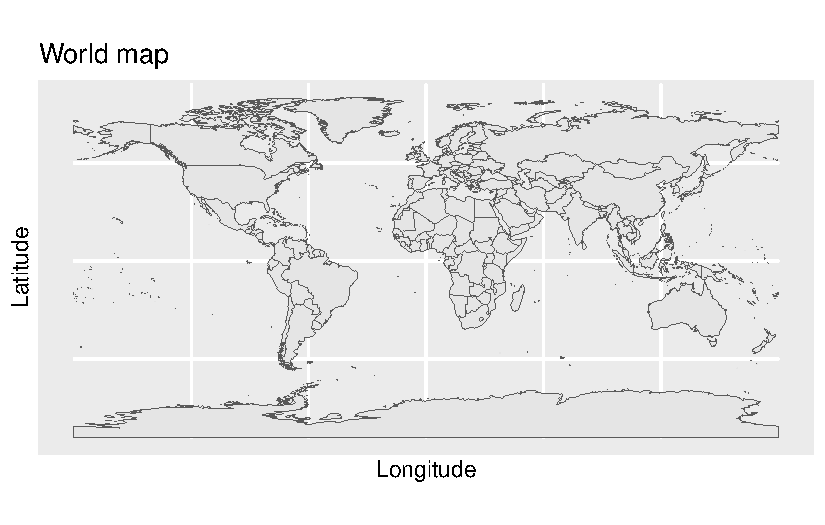
\includegraphics{Introduction-to-mapping_files/figure-pdf/unnamed-chunk-7-1.pdf}

}

\end{figure}

\hypertarget{map-color-geom_sf}{%
\subsection{\texorpdfstring{Map color
(\texttt{geom\_sf})}{Map color (geom\_sf)}}\label{map-color-geom_sf}}

In many ways, \texttt{sf} geometries are no different than regular
geometries, and can be displayed with the same level of control on their
attributes. Here is an example with the polygons of the countries filled
with a green color (argument \texttt{fill}), using black for the outline
of the countries (argument \texttt{color}):

\begin{Shaded}
\begin{Highlighting}[]
\CommentTok{\#|label: showing colour and fill}
\FunctionTok{ggplot}\NormalTok{(}\AttributeTok{data =}\NormalTok{ world) }\SpecialCharTok{+}      
  \FunctionTok{geom\_sf}\NormalTok{(}\AttributeTok{color =} \StringTok{"black"}\NormalTok{, }\AttributeTok{fill =} \StringTok{"lightgreen"}\NormalTok{)}
\end{Highlighting}
\end{Shaded}

\begin{figure}[H]

{\centering 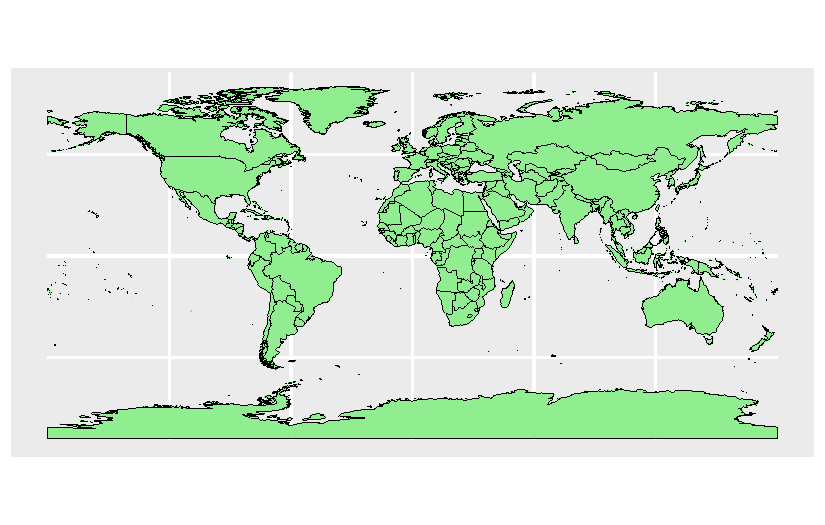
\includegraphics{Introduction-to-mapping_files/figure-pdf/unnamed-chunk-8-1.pdf}

}

\end{figure}

\begin{Shaded}
\begin{Highlighting}[]
\CommentTok{\# now lets make two layers, one for NZ, that is different coloured.}
\FunctionTok{ggplot}\NormalTok{() }\SpecialCharTok{+}      
  \FunctionTok{geom\_sf}\NormalTok{(}\AttributeTok{data =}\NormalTok{ world, }\AttributeTok{color =} \StringTok{"black"}\NormalTok{, }\AttributeTok{fill =} \StringTok{"lightgreen"}\NormalTok{) }\SpecialCharTok{+}
  \FunctionTok{geom\_sf}\NormalTok{(}\AttributeTok{data =}\NormalTok{ nz, }\AttributeTok{color =} \StringTok{"black"}\NormalTok{, }\AttributeTok{fill =} \StringTok{"blue"}\NormalTok{)}
\end{Highlighting}
\end{Shaded}

\begin{figure}[H]

{\centering 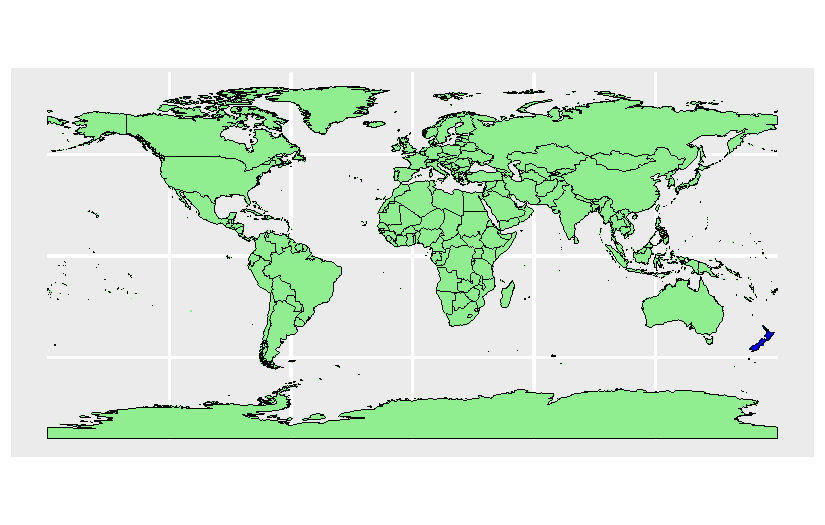
\includegraphics{Introduction-to-mapping_files/figure-pdf/unnamed-chunk-8-2.pdf}

}

\end{figure}

The package \texttt{ggplot2} allows the use of more complex color
schemes, such as a gradient on one variable of the data. Here is another
example that shows the population of each country. In this example, we
use the ``viridis'' colorblind-friendly palette for the color gradient
(with \texttt{option\ =\ "plasma"} for the plasma variant), using the
square root of the population (which is stored in the variable
\texttt{POP\_EST} of the \texttt{world} object):

\begin{Shaded}
\begin{Highlighting}[]
\CommentTok{\#|label: other fill alternatives}
\FunctionTok{ggplot}\NormalTok{(}\AttributeTok{data =}\NormalTok{ world) }\SpecialCharTok{+}     
  \FunctionTok{geom\_sf}\NormalTok{(}\FunctionTok{aes}\NormalTok{(}\AttributeTok{fill =}\NormalTok{ pop\_est)) }\SpecialCharTok{+}     
  \FunctionTok{scale\_fill\_viridis\_c}\NormalTok{(}\AttributeTok{option =} \StringTok{"plasma"}\NormalTok{, }\AttributeTok{trans =} \StringTok{"sqrt"}\NormalTok{) }
\end{Highlighting}
\end{Shaded}

\begin{figure}[H]

{\centering 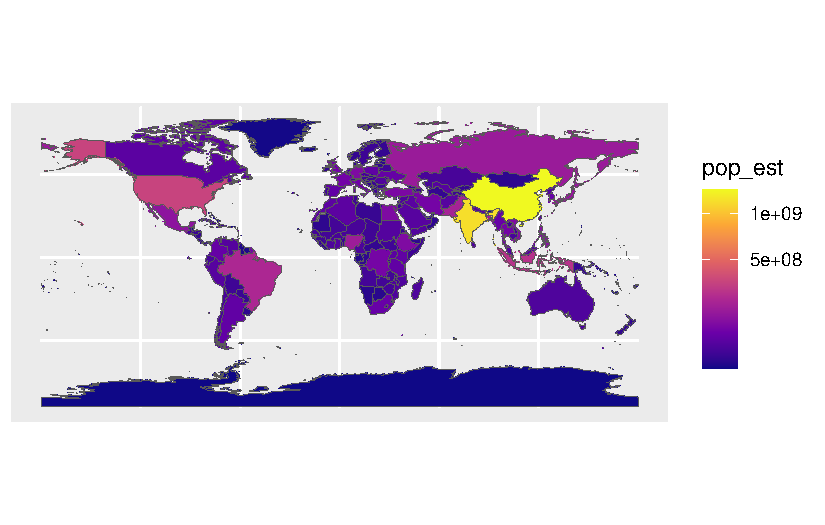
\includegraphics{Introduction-to-mapping_files/figure-pdf/unnamed-chunk-9-1.pdf}

}

\end{figure}

\hypertarget{projection-and-extent-coord_sf}{%
\subsection{\texorpdfstring{Projection and extent
(\texttt{coord\_sf})}{Projection and extent (coord\_sf)}}\label{projection-and-extent-coord_sf}}

The function \texttt{coord\_sf} allows to deal with the coordinate
system, which includes both projection and extent of the map. By
default, the map will use the coordinate system of the first layer that
defines one (i.e.~scanned in the order provided), or if none, fall back
on WGS84 (latitude/longitude, the reference system used in GPS). Using
the argument \texttt{crs}, it is possible to override this setting, and
project on the fly to any projection. This can be achieved using any
valid PROJ4 string (here, the European-centric ETRS89 Lambert Azimuthal
Equal-Area projection):

Note on Coordinate Reference System (CRS) determines the location that
points are placed on a plot

\begin{Shaded}
\begin{Highlighting}[]
\CommentTok{\#|label: }
\FunctionTok{ggplot}\NormalTok{(}\AttributeTok{data =}\NormalTok{ world) }\SpecialCharTok{+}     
  \FunctionTok{geom\_sf}\NormalTok{() }\SpecialCharTok{+}     
  \FunctionTok{coord\_sf}\NormalTok{(}\AttributeTok{crs =} \StringTok{"+proj=laea +lat\_0=52 +lon\_0=10 +x\_0=4321000 +y\_0=3210000 +ellps=GRS80 +units=m +no\_defs "}\NormalTok{)}
\end{Highlighting}
\end{Shaded}

\begin{figure}[H]

{\centering 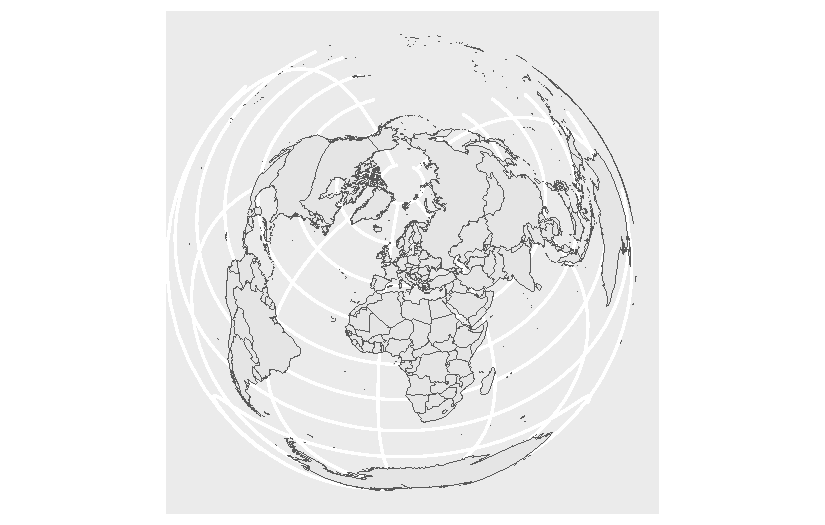
\includegraphics{Introduction-to-mapping_files/figure-pdf/unnamed-chunk-10-1.pdf}

}

\end{figure}

Spatial Reference System Identifier (SRID) or an European Petroleum
Survey Group (EPSG) code are available for the projection of interest,
they can be used directly instead of the full PROJ4 string. The two
following calls are equivalent for the ETRS89 Lambert Azimuthal
Equal-Area projection, which is EPSG code 3035:

\begin{Shaded}
\begin{Highlighting}[]
\CommentTok{\#|label: shortened CRS }
\FunctionTok{ggplot}\NormalTok{(}\AttributeTok{data =}\NormalTok{ world) }\SpecialCharTok{+}     
  \FunctionTok{geom\_sf}\NormalTok{() }\SpecialCharTok{+}     
  \FunctionTok{coord\_sf}\NormalTok{(}\AttributeTok{crs =} \StringTok{"+init=epsg:3035"}\NormalTok{)  }
\end{Highlighting}
\end{Shaded}

\begin{verbatim}
Warning in CPL_crs_from_input(x): GDAL Message 1: +init=epsg:XXXX syntax is
deprecated. It might return a CRS with a non-EPSG compliant axis order.
\end{verbatim}

\begin{figure}[H]

{\centering 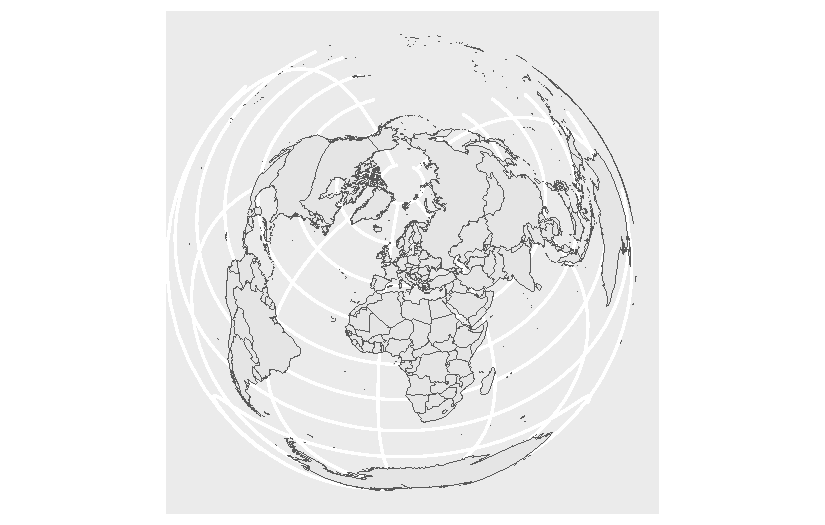
\includegraphics{Introduction-to-mapping_files/figure-pdf/unnamed-chunk-11-1.pdf}

}

\end{figure}

\begin{Shaded}
\begin{Highlighting}[]
\FunctionTok{ggplot}\NormalTok{(}\AttributeTok{data =}\NormalTok{ world) }\SpecialCharTok{+}     
  \FunctionTok{geom\_sf}\NormalTok{() }\SpecialCharTok{+}     
  \FunctionTok{coord\_sf}\NormalTok{(}\AttributeTok{crs =} \FunctionTok{st\_crs}\NormalTok{(}\DecValTok{3035}\NormalTok{)) }
\end{Highlighting}
\end{Shaded}

\begin{figure}[H]

{\centering 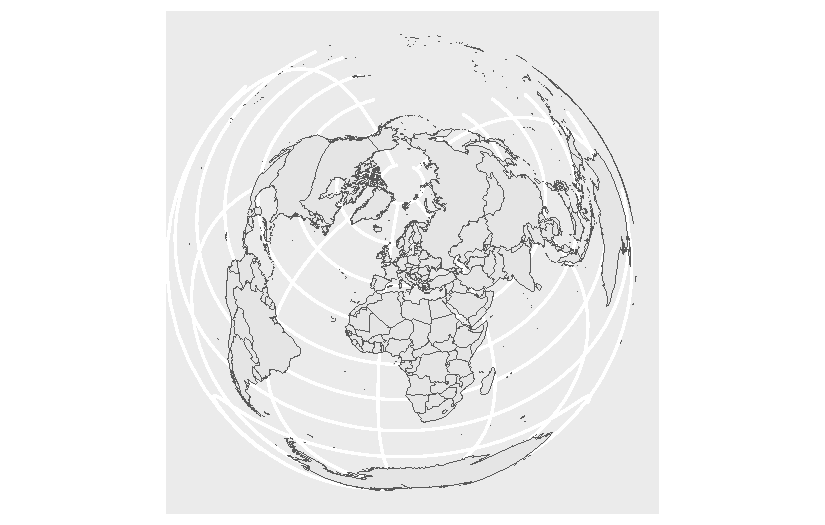
\includegraphics{Introduction-to-mapping_files/figure-pdf/unnamed-chunk-11-2.pdf}

}

\end{figure}

The extent of the map can also be set in \texttt{coord\_sf}, in practice
allowing to ``zoom'' in the area of interest, provided by limits on the
x-axis (\texttt{xlim}), and on the y-axis (\texttt{ylim}). Note that the
limits are automatically expanded by a fraction to ensure that data and
axes don't overlap; it can also be turned off to exactly match the
limits provided with \texttt{expand\ =\ FALSE}:

\begin{Shaded}
\begin{Highlighting}[]
\CommentTok{\#|label: zooming on a map}

\FunctionTok{ggplot}\NormalTok{(}\AttributeTok{data =}\NormalTok{ world) }\SpecialCharTok{+}     
  \FunctionTok{geom\_sf}\NormalTok{() }\SpecialCharTok{+}     
  \FunctionTok{coord\_sf}\NormalTok{(}\AttributeTok{xlim =} \FunctionTok{c}\NormalTok{(}\SpecialCharTok{{-}}\FloatTok{102.15}\NormalTok{, }\SpecialCharTok{{-}}\FloatTok{74.12}\NormalTok{), }
           \AttributeTok{ylim =} \FunctionTok{c}\NormalTok{(}\FloatTok{7.65}\NormalTok{, }\FloatTok{33.97}\NormalTok{), }
           \AttributeTok{expand =} \ConstantTok{FALSE}
\NormalTok{           ) }
\end{Highlighting}
\end{Shaded}

\begin{figure}[H]

{\centering 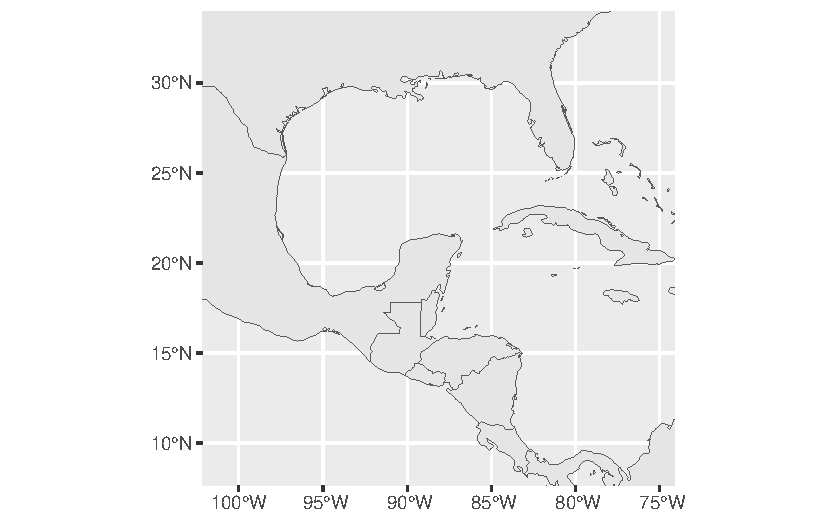
\includegraphics{Introduction-to-mapping_files/figure-pdf/unnamed-chunk-12-1.pdf}

}

\end{figure}

\hypertarget{scale-bar-and-north-arrow-package-ggspatial}{%
\subsection{\texorpdfstring{Scale bar and North arrow (package
\texttt{ggspatial})}{Scale bar and North arrow (package ggspatial)}}\label{scale-bar-and-north-arrow-package-ggspatial}}

Several packages are available to create a scale bar on a map
(e.g.~\texttt{prettymapr}, \texttt{vcd}, \texttt{ggsn}, or
\texttt{legendMap}). We introduce here the package \texttt{ggspatial},
which provides easy-to-use functions\ldots{}

\texttt{scale\_bar} that allows to add simultaneously the north symbol
and a scale bar into the \texttt{ggplot} map. Five arguments need to be
set manually: \texttt{lon}, \texttt{lat}, \texttt{distance\_lon},
\texttt{distance\_lat}, and \texttt{distance\_legend}. The location of
the scale bar has to be specified in longitude/latitude in the
\texttt{lon} and \texttt{lat} arguments. The shaded distance inside the
scale bar is controlled by the \texttt{distance\_lon} argument. while
its width is determined by \texttt{distance\_lat}. Additionally, it is
possible to change the font size for the legend of the scale bar
(argument \texttt{legend\_size}, which defaults to 3). The North arrow
behind the ``N'' north symbol can also be adjusted for its length
(\texttt{arrow\_length}), its distance to the scale
(\texttt{arrow\_distance}), or the size the N north symbol itself
(\texttt{arrow\_north\_size}, which defaults to 6). Note that all
distances (\texttt{distance\_lon}, \texttt{distance\_lat},
\texttt{distance\_legend}, \texttt{arrow\_length},
\texttt{arrow\_distance}) are set to \texttt{"km"} by default in
\texttt{distance\_unit}; they can also be set to nautical miles with
``nm'', or miles with ``mi''.

\begin{Shaded}
\begin{Highlighting}[]
\CommentTok{\#|label: adding North arrow and scale bar}
\FunctionTok{library}\NormalTok{(}\StringTok{"ggspatial"}\NormalTok{) }

\FunctionTok{ggplot}\NormalTok{(}\AttributeTok{data =}\NormalTok{ world) }\SpecialCharTok{+}     
  \FunctionTok{geom\_sf}\NormalTok{() }\SpecialCharTok{+}     
  \FunctionTok{annotation\_scale}\NormalTok{(}\AttributeTok{location =} \StringTok{"bl"}\NormalTok{, }\AttributeTok{width\_hint =} \FloatTok{0.5}\NormalTok{) }\SpecialCharTok{+}     
  \FunctionTok{annotation\_north\_arrow}\NormalTok{(}\AttributeTok{location =} \StringTok{"bl"}\NormalTok{, }
                         \AttributeTok{which\_north =} \StringTok{"true"}\NormalTok{,          }
                         \AttributeTok{pad\_x =} \FunctionTok{unit}\NormalTok{(}\FloatTok{0.75}\NormalTok{, }\StringTok{"in"}\NormalTok{), }
                         \AttributeTok{pad\_y =} \FunctionTok{unit}\NormalTok{(}\FloatTok{0.5}\NormalTok{, }\StringTok{"in"}\NormalTok{),         }
                         \AttributeTok{style =}\NormalTok{ north\_arrow\_fancy\_orienteering) }\SpecialCharTok{+}     
  \FunctionTok{coord\_sf}\NormalTok{(}\AttributeTok{xlim =} \FunctionTok{c}\NormalTok{(}\SpecialCharTok{{-}}\FloatTok{102.15}\NormalTok{, }\SpecialCharTok{{-}}\FloatTok{74.12}\NormalTok{), }\AttributeTok{ylim =} \FunctionTok{c}\NormalTok{(}\FloatTok{7.65}\NormalTok{, }\FloatTok{33.97}\NormalTok{))  }
\end{Highlighting}
\end{Shaded}

\begin{verbatim}
Scale on map varies by more than 10%, scale bar may be inaccurate
\end{verbatim}

\begin{figure}[H]

{\centering 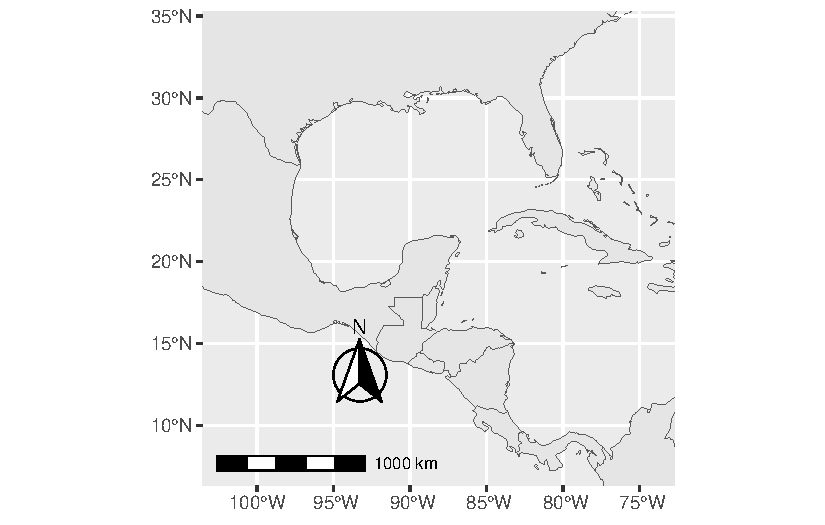
\includegraphics{Introduction-to-mapping_files/figure-pdf/unnamed-chunk-13-1.pdf}

}

\end{figure}

\begin{Shaded}
\begin{Highlighting}[]
\DocumentationTok{\#\# Scale on map varies by more than 10\%, scale bar may be inaccurate }
\end{Highlighting}
\end{Shaded}

Note the warning of the inaccurate scale bar: since the map use
unprojected data in longitude/latitude (WGS84) on an equidistant
cylindrical projection (all meridians being parallel), length in
(kilo)meters on the map directly depends mathematically on the degree of
latitude. Plots of small regions or projected data will often allow for
more accurate scale bars.

\hypertarget{country-names-and-other-names-geom_text-and-annotate}{%
\subsection{\texorpdfstring{Country names and other names
(\texttt{geom\_text} and
\texttt{annotate})}{Country names and other names (geom\_text and annotate)}}\label{country-names-and-other-names-geom_text-and-annotate}}

The \texttt{world} data set already contains country names and the
coordinates of the centroid of each country (among more information). We
can use this information to plot country names, using \texttt{world} as
a regular \texttt{data.frame} in \texttt{ggplot2}. The function
\texttt{geom\_text} can be used to add a layer of text to a map using
geographic coordinates. The function requires the data needed to enter
the country names, which is the same data as the world map. Again, we
have a very flexible control to adjust the text at will on many aspects:

\begin{itemize}
\tightlist
\item
  The size (argument \texttt{size});
\item
  The alignment, which is centered by default on the coordinates
  provided. The text can be adjusted horizontally or vertically using
  the arguments \texttt{hjust} and \texttt{vjust}, which can either be a
  number between 0 (right/bottom) and 1 (top/left) or a character
  (``left'', ``middle'', ``right'', ``bottom'', ``center'', ``top'').
  The text can also be offset horizontally or vertically with the
  argument \texttt{nudge\_x} and \texttt{nudge\_y};
\item
  The font of the text, for instance its color (argument \texttt{color})
  or the type of font (\texttt{fontface});
\item
  The overlap of labels, using the argument \texttt{check\_overlap},
  which removes overlapping text. Alternatively, when there is a lot of
  overlapping labels, the package \texttt{ggrepel} provides a
  \texttt{geom\_text\_repel} function that moves label around so that
  they do not overlap.
\item
  For the text labels, we are defining the centroid of the counties with
  \texttt{st\_centroid}, from the package \texttt{sf}. Then we combined
  the coordinates with the centroid, in the \texttt{geometry} of the
  spatial data frame. The package \texttt{sf} is necessary for the
  command \texttt{st\_centroid}.
\end{itemize}

Define centroid! The centre of a polygon i.e.~a country/shape on a map

Additionally, the \texttt{annotate} function can be used to add a single
character string at a specific location, as demonstrated here to add the
Gulf of Mexico:

\begin{Shaded}
\begin{Highlighting}[]
\CommentTok{\#|label: adding centroids}
\CommentTok{\#|warnings: false}
\CommentTok{\#|error: false}

\FunctionTok{library}\NormalTok{(}\StringTok{"sf"}\NormalTok{) }

\NormalTok{world }\OtherTok{\textless{}{-}} \FunctionTok{st\_make\_valid}\NormalTok{(world) }\CommentTok{\# this is an additional step needed because the centroids could not be computed  }
\NormalTok{world\_points}\OtherTok{\textless{}{-}} \FunctionTok{st\_centroid}\NormalTok{(world) }
\end{Highlighting}
\end{Shaded}

\begin{verbatim}
Warning: st_centroid assumes attributes are constant over geometries
\end{verbatim}

\begin{Shaded}
\begin{Highlighting}[]
\NormalTok{world\_points }\OtherTok{\textless{}{-}} \FunctionTok{cbind}\NormalTok{(world, }\FunctionTok{st\_coordinates}\NormalTok{(}\FunctionTok{st\_centroid}\NormalTok{(world}\SpecialCharTok{$}\NormalTok{geometry)))  }

\FunctionTok{ggplot}\NormalTok{(}\AttributeTok{data =}\NormalTok{ world) }\SpecialCharTok{+} 
  \FunctionTok{geom\_sf}\NormalTok{() }\SpecialCharTok{+} 
  \FunctionTok{geom\_text}\NormalTok{(}\AttributeTok{data=}\NormalTok{ world\_points,}
            \FunctionTok{aes}\NormalTok{(}\AttributeTok{x=}\NormalTok{X, }\AttributeTok{y=}\NormalTok{Y, }\AttributeTok{label=}\NormalTok{name),     }
            \AttributeTok{color =} \StringTok{"darkblue"}\NormalTok{, }
            \AttributeTok{fontface =} \StringTok{"bold"}\NormalTok{, }
            \AttributeTok{check\_overlap =} \ConstantTok{FALSE}\NormalTok{) }\SpecialCharTok{+} 
  \FunctionTok{annotate}\NormalTok{(}\AttributeTok{geom =} \StringTok{"text"}\NormalTok{, }
           \AttributeTok{x =} \SpecialCharTok{{-}}\DecValTok{90}\NormalTok{, }
           \AttributeTok{y =} \DecValTok{26}\NormalTok{, }
           \AttributeTok{label =} \StringTok{"Gulf of Mexico"}\NormalTok{,      }
           \AttributeTok{fontface =} \StringTok{"italic"}\NormalTok{, }
           \AttributeTok{color =} \StringTok{"grey22"}\NormalTok{, }
           \AttributeTok{size =} \DecValTok{6}\NormalTok{) }\SpecialCharTok{+} 
  \FunctionTok{coord\_sf}\NormalTok{(}\AttributeTok{xlim =} \FunctionTok{c}\NormalTok{(}\SpecialCharTok{{-}}\FloatTok{102.15}\NormalTok{, }\SpecialCharTok{{-}}\FloatTok{74.12}\NormalTok{), }
           \AttributeTok{ylim =} \FunctionTok{c}\NormalTok{(}\FloatTok{7.65}\NormalTok{, }\FloatTok{33.97}\NormalTok{), }
           \AttributeTok{expand =} \ConstantTok{FALSE}\NormalTok{) }
\end{Highlighting}
\end{Shaded}

\begin{figure}[H]

{\centering 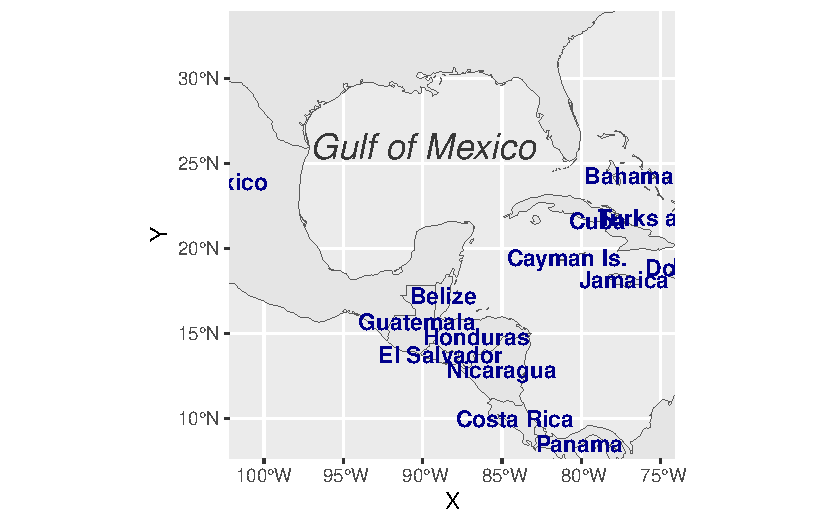
\includegraphics{Introduction-to-mapping_files/figure-pdf/unnamed-chunk-14-1.pdf}

}

\end{figure}

\hypertarget{final-map}{%
\section{Final map}\label{final-map}}

Now to make the final touches, the theme of the map can be edited to
make it more appealing. We suggested the use of \texttt{theme\_bw} for a
standard theme, but there are many other themes that can be selected
from (see for instance \texttt{?ggtheme} in \texttt{ggplot2}, or the
package
\href{https://cran.r-project.org/package=ggthemes}{\texttt{ggthemes}}
which provide several useful themes). Moreover, specific theme elements
can be tweaked to get to the final outcome:

\begin{itemize}
\tightlist
\item
  Position of the legend: Although not used in this example, the
  argument \texttt{legend.position} allows to automatically place the
  legend at a specific location (e.g.~\texttt{"topright"},
  \texttt{"bottomleft"}, etc.);
\item
  Grid lines (graticules) on the map: by using \texttt{panel.grid.major}
  and \texttt{panel.grid.minor}, grid lines can be adjusted. Here we set
  them to a gray color and dashed line type to clearly distinguish them
  from country borders lines;
\item
  Map background: the argument \texttt{panel.background} can be used to
  color the background, which is the ocean essentially, with a light
  blue;
\item
  Many more elements of a theme can be adjusted, which would be too long
  to cover here. We refer the reader to the documentation for the
  function \texttt{theme}.
\end{itemize}

\begin{Shaded}
\begin{Highlighting}[]
\CommentTok{\#|label: cool as map}

\FunctionTok{ggplot}\NormalTok{(}\AttributeTok{data =}\NormalTok{ world) }\SpecialCharTok{+} 
  \FunctionTok{geom\_sf}\NormalTok{(}\AttributeTok{fill=} \StringTok{"antiquewhite"}\NormalTok{) }\SpecialCharTok{+} 
  \FunctionTok{geom\_text}\NormalTok{(}\AttributeTok{data=}\NormalTok{ world\_points,}
            \FunctionTok{aes}\NormalTok{(}\AttributeTok{x=}\NormalTok{X, }
                \AttributeTok{y=}\NormalTok{Y, }
                \AttributeTok{label=}\NormalTok{name), }
            \AttributeTok{color =} \StringTok{"darkblue"}\NormalTok{, }
            \AttributeTok{fontface =} \StringTok{"bold"}\NormalTok{, }
            \AttributeTok{check\_overlap =} \ConstantTok{FALSE}\NormalTok{) }\SpecialCharTok{+} 
  \FunctionTok{annotate}\NormalTok{(}\AttributeTok{geom =} \StringTok{"text"}\NormalTok{, }
           \AttributeTok{x =} \SpecialCharTok{{-}}\DecValTok{90}\NormalTok{, }
           \AttributeTok{y =} \DecValTok{26}\NormalTok{, }
           \AttributeTok{label =} \StringTok{"Gulf of Mexico"}\NormalTok{, }
           \AttributeTok{fontface =} \StringTok{"italic"}\NormalTok{, }
           \AttributeTok{color =} \StringTok{"grey22"}\NormalTok{, }
           \AttributeTok{size =} \DecValTok{6}\NormalTok{) }\SpecialCharTok{+} 
  \FunctionTok{annotation\_scale}\NormalTok{(}\AttributeTok{location =} \StringTok{"bl"}\NormalTok{, }
                   \AttributeTok{width\_hint =} \FloatTok{0.5}\NormalTok{) }\SpecialCharTok{+} 
  \FunctionTok{annotation\_north\_arrow}\NormalTok{(}\AttributeTok{location =} \StringTok{"bl"}\NormalTok{, }
                         \AttributeTok{which\_north =} \StringTok{"true"}\NormalTok{, }
                         \AttributeTok{pad\_x =} \FunctionTok{unit}\NormalTok{(}\FloatTok{0.75}\NormalTok{, }\StringTok{"in"}\NormalTok{), }
                         \AttributeTok{pad\_y =} \FunctionTok{unit}\NormalTok{(}\FloatTok{0.5}\NormalTok{, }\StringTok{"in"}\NormalTok{), }
                         \AttributeTok{style =}\NormalTok{ north\_arrow\_fancy\_orienteering) }\SpecialCharTok{+} 
  \FunctionTok{coord\_sf}\NormalTok{(}\AttributeTok{xlim =} \FunctionTok{c}\NormalTok{(}\SpecialCharTok{{-}}\FloatTok{102.15}\NormalTok{, }\SpecialCharTok{{-}}\FloatTok{74.12}\NormalTok{), }
           \AttributeTok{ylim =} \FunctionTok{c}\NormalTok{(}\FloatTok{7.65}\NormalTok{, }\FloatTok{33.97}\NormalTok{), }
           \AttributeTok{expand =} \ConstantTok{FALSE}\NormalTok{) }\SpecialCharTok{+} 
  \FunctionTok{xlab}\NormalTok{(}\StringTok{"Longitude"}\NormalTok{) }\SpecialCharTok{+} 
  \FunctionTok{ylab}\NormalTok{(}\StringTok{"Latitude"}\NormalTok{) }\SpecialCharTok{+} 
  \FunctionTok{ggtitle}\NormalTok{(}\StringTok{"Map of the Gulf of Mexico and the Caribbean Sea"}\NormalTok{) }
\end{Highlighting}
\end{Shaded}

\begin{verbatim}
Scale on map varies by more than 10%, scale bar may be inaccurate
\end{verbatim}

\begin{figure}[H]

{\centering 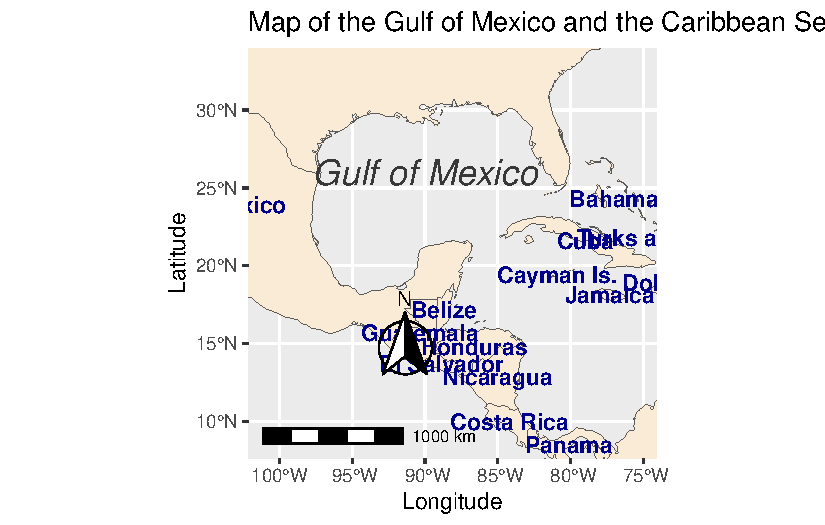
\includegraphics{Introduction-to-mapping_files/figure-pdf/unnamed-chunk-15-1.pdf}

}

\end{figure}

\hypertarget{saving-the-map-with-ggsave}{%
\subsection{\texorpdfstring{Saving the map with
\texttt{ggsave}}{Saving the map with ggsave}}\label{saving-the-map-with-ggsave}}

The final map now ready, it is very easy to save it using
\texttt{ggsave}. This function allows a graphic (typically the last plot
displayed) to be saved in a variety of formats, including the most
common PNG (raster bitmap) and PDF (vector graphics), with control over
the size and resolution of the outcome. For instance here, we save a PDF
version of the map, which keeps the best quality, and a PNG version of
it for web purposes:

\begin{Shaded}
\begin{Highlighting}[]
\CommentTok{\#|label: our old friend ggsave}
\CommentTok{\#| eval: false}
\CommentTok{\#| echo: true }

\CommentTok{\# ggsave("map.pdf")}
\CommentTok{\# ggsave("map\_web.png",}
\CommentTok{\#        width = 6,}
\CommentTok{\#        height = 6,}
\CommentTok{\#        dpi = "screen")}
\end{Highlighting}
\end{Shaded}

\hypertarget{a-kiwi-applicaiton}{%
\subsection{A kiwi applicaiton}\label{a-kiwi-applicaiton}}

As an example of your new found wisdom lets create a map of the
universities found in New Zealand using the sf package and ggplot.

\begin{Shaded}
\begin{Highlighting}[]
\FunctionTok{library}\NormalTok{(tidyverse)}
\FunctionTok{library}\NormalTok{(sf)}
\FunctionTok{library}\NormalTok{(ggrepel)}
\FunctionTok{library}\NormalTok{(ggthemes)}
\FunctionTok{library}\NormalTok{(here) }\CommentTok{\# make a note of this package}
\end{Highlighting}
\end{Shaded}

Here() is a new package we haven't come across yet, it is used to find
the path to our working directory which can be useful when we need to
tell R exactly where something is on our machine.

The sf mapping workflow: - format inputs - call data - add layers

download from https://data.linz.govt.nz/ you need to create an account,
can be hard to find the rights layers, it can also take time to prepare
the download for you or, get from my GitHub

\begin{Shaded}
\begin{Highlighting}[]
\CommentTok{\#|label: import of nz data data}
\FunctionTok{library}\NormalTok{(here)}
\end{Highlighting}
\end{Shaded}

\begin{verbatim}
here() starts at C:/Users/MarmontB/OneDrive - DairyNZ Limited/Documents/R/waikato_r4ds_2023
\end{verbatim}

\begin{Shaded}
\begin{Highlighting}[]
\NormalTok{?}\FunctionTok{here}\NormalTok{()}
\end{Highlighting}
\end{Shaded}

\begin{verbatim}
starting httpd help server ...
\end{verbatim}

\begin{verbatim}
 done
\end{verbatim}

\begin{Shaded}
\begin{Highlighting}[]
\NormalTok{file\_path }\OtherTok{\textless{}{-}} \StringTok{"C:/Users/MarmontB/OneDrive {-} DairyNZ Limited/Documents/R/waikato\_r4ds\_2023/Week 13/Smorgasbord/nz{-}coastlines{-}and{-}islands{-}polygons{-}topo{-}150k"}
\NormalTok{nz\_outline }\OtherTok{\textless{}{-}} \FunctionTok{st\_read}\NormalTok{(file\_path)}
\end{Highlighting}
\end{Shaded}

\begin{verbatim}
Reading layer `nz-coastlines-and-islands-polygons-topo-150k' from data source 
  `C:\Users\MarmontB\OneDrive - DairyNZ Limited\Documents\R\waikato_r4ds_2023\Week 13\Smorgasbord\nz-coastlines-and-islands-polygons-topo-150k' 
  using driver `ESRI Shapefile'
Simple feature collection with 9131 features and 7 fields
Geometry type: POLYGON
Dimension:     XY
Bounding box:  xmin: 165.869 ymin: -52.62088 xmax: 183.8457 ymax: -29.23134
Geodetic CRS:  NZGD2000
\end{verbatim}

\begin{Shaded}
\begin{Highlighting}[]
\CommentTok{\# we can use the here function to reduce the copy and pasting!}
\NormalTok{file\_path }\OtherTok{\textless{}{-}} \FunctionTok{here}\NormalTok{(}\StringTok{"Week 13"}\NormalTok{, }\StringTok{"Smorgasbord"}\NormalTok{, }\StringTok{"nz{-}coastlines{-}and{-}islands{-}polygons{-}topo{-}150k"}\NormalTok{)}
\NormalTok{nz\_outline }\OtherTok{\textless{}{-}} \FunctionTok{st\_read}\NormalTok{(file\_path)}
\end{Highlighting}
\end{Shaded}

\begin{verbatim}
Reading layer `nz-coastlines-and-islands-polygons-topo-150k' from data source 
  `C:\Users\MarmontB\OneDrive - DairyNZ Limited\Documents\R\waikato_r4ds_2023\Week 13\Smorgasbord\nz-coastlines-and-islands-polygons-topo-150k' 
  using driver `ESRI Shapefile'
Simple feature collection with 9131 features and 7 fields
Geometry type: POLYGON
Dimension:     XY
Bounding box:  xmin: 165.869 ymin: -52.62088 xmax: 183.8457 ymax: -29.23134
Geodetic CRS:  NZGD2000
\end{verbatim}

\begin{Shaded}
\begin{Highlighting}[]
\CommentTok{\# file\_path \textless{}{-} "C:/Users/MarmontB/OneDrive {-} DairyNZ Limited/Documents/R/waikato\_r4ds\_2023/Week 13/Smorgasbord/nz{-}land{-}districts"}
\NormalTok{file\_path }\OtherTok{\textless{}{-}} \FunctionTok{here}\NormalTok{(}\StringTok{"Week 13"}\NormalTok{, }\StringTok{"Smorgasbord"}\NormalTok{, }\StringTok{"nz{-}land{-}districts"}\NormalTok{)}
\NormalTok{nz\_regions }\OtherTok{\textless{}{-}} \FunctionTok{st\_read}\NormalTok{(file\_path)}
\end{Highlighting}
\end{Shaded}

\begin{verbatim}
Reading layer `nz-land-districts' from data source 
  `C:\Users\MarmontB\OneDrive - DairyNZ Limited\Documents\R\waikato_r4ds_2023\Week 13\Smorgasbord\nz-land-districts' 
  using driver `ESRI Shapefile'
Simple feature collection with 12 features and 2 fields
Geometry type: MULTIPOLYGON
Dimension:     XY
Bounding box:  xmin: 166.1345 ymin: -47.73475 xmax: 184.5 ymax: -33.99975
Geodetic CRS:  NZGD2000
\end{verbatim}

\begin{Shaded}
\begin{Highlighting}[]
\CommentTok{\# The location of NZUs comes from google maps, can demonstrate}
\NormalTok{NZUs }\OtherTok{\textless{}{-}} \FunctionTok{tibble}\NormalTok{(}\AttributeTok{Universities =} \FunctionTok{c}\NormalTok{(}\StringTok{"UoA"}\NormalTok{, }\StringTok{"AUT"}\NormalTok{, }\StringTok{"Waikato"}\NormalTok{, }\StringTok{"Massey"}\NormalTok{, }\StringTok{"Vic"}\NormalTok{, }\StringTok{"Canterbury"}\NormalTok{, }\StringTok{"Lincoln"}\NormalTok{, }\StringTok{"Otago"}\NormalTok{),}
               \AttributeTok{lat =} \FunctionTok{c}\NormalTok{(}\SpecialCharTok{{-}}\FloatTok{36.85224823346041}\NormalTok{, }\SpecialCharTok{{-}}\FloatTok{36.853412307817784}\NormalTok{, }\SpecialCharTok{{-}}\FloatTok{37.78890569065363}\NormalTok{, }\SpecialCharTok{{-}}\FloatTok{40.355225055311955}\NormalTok{, }\SpecialCharTok{{-}}\FloatTok{41.29002684516775}\NormalTok{, }\SpecialCharTok{{-}}\FloatTok{43.52237464482431}\NormalTok{, }\SpecialCharTok{{-}}\FloatTok{43.645401275754104}\NormalTok{, }\SpecialCharTok{{-}}\FloatTok{45.864063192916205}\NormalTok{),}
               \AttributeTok{lng =} \FunctionTok{c}\NormalTok{(}\FloatTok{174.77252663829262}\NormalTok{, }\FloatTok{174.76643757919567}\NormalTok{, }\FloatTok{175.3164528404978}\NormalTok{, }\FloatTok{175.60943830584307}\NormalTok{,}\FloatTok{174.76783598210622}\NormalTok{, }\FloatTok{172.57943539626334}\NormalTok{, }\FloatTok{172.46426811709463}\NormalTok{, }\FloatTok{170.5146851684737}\NormalTok{))  }\SpecialCharTok{|\textgreater{}}  
  \FunctionTok{select}\NormalTok{(Universities, lng, lat)}
\end{Highlighting}
\end{Shaded}

\begin{Shaded}
\begin{Highlighting}[]
\CommentTok{\#|label: create basic nz maps}
\FunctionTok{ggplot}\NormalTok{(}\AttributeTok{data =}\NormalTok{ nz\_regions) }\SpecialCharTok{+}
  \FunctionTok{geom\_sf}\NormalTok{()}
\end{Highlighting}
\end{Shaded}

\begin{figure}[H]

{\centering 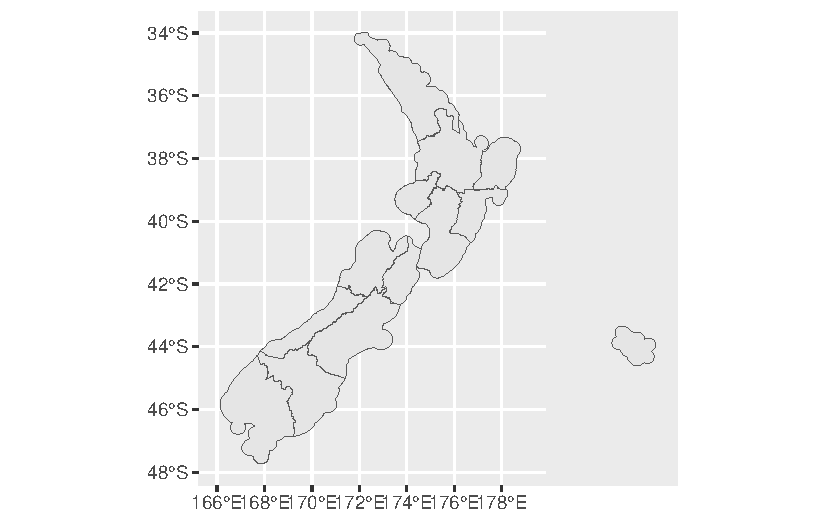
\includegraphics{Introduction-to-mapping_files/figure-pdf/unnamed-chunk-19-1.pdf}

}

\end{figure}

\begin{Shaded}
\begin{Highlighting}[]
\FunctionTok{ggplot}\NormalTok{(nz\_outline) }\SpecialCharTok{+}
  \FunctionTok{geom\_sf}\NormalTok{()}
\end{Highlighting}
\end{Shaded}

\begin{figure}[H]

{\centering 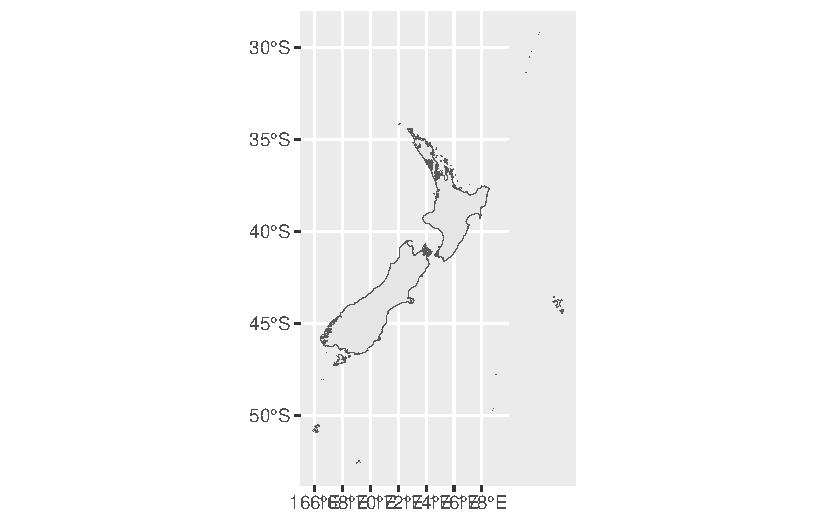
\includegraphics{Introduction-to-mapping_files/figure-pdf/unnamed-chunk-19-2.pdf}

}

\end{figure}

\begin{Shaded}
\begin{Highlighting}[]
\CommentTok{\# note that the region map has fluffy borders}
\end{Highlighting}
\end{Shaded}

\begin{Shaded}
\begin{Highlighting}[]
\NormalTok{trimmed }\OtherTok{\textless{}{-}} \FunctionTok{st\_intersection}\NormalTok{(nz\_outline, nz\_regions)}
\end{Highlighting}
\end{Shaded}

\begin{verbatim}
Warning: attribute variables are assumed to be spatially constant throughout
all geometries
\end{verbatim}

\begin{Shaded}
\begin{Highlighting}[]
\FunctionTok{ggplot}\NormalTok{(}\AttributeTok{data =}\NormalTok{ trimmed) }\SpecialCharTok{+}
  \FunctionTok{geom\_sf}\NormalTok{()}
\end{Highlighting}
\end{Shaded}

\begin{figure}[H]

{\centering 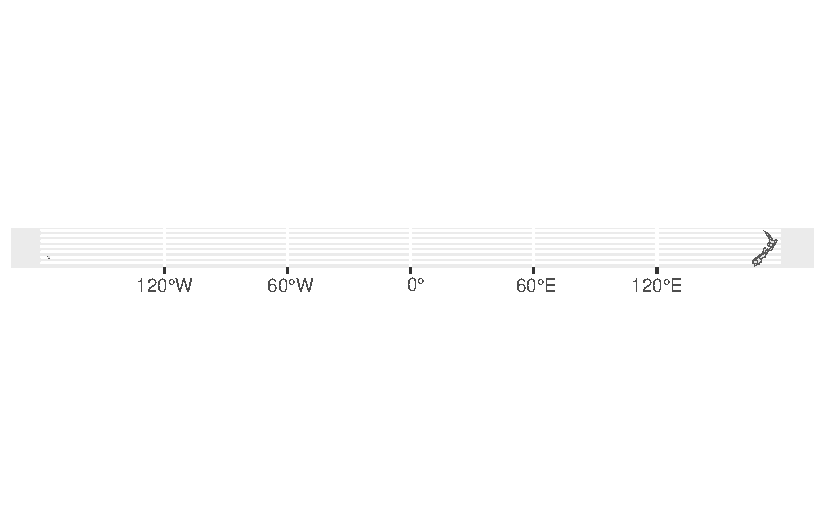
\includegraphics{Introduction-to-mapping_files/figure-pdf/making tighter map-1.pdf}

}

\end{figure}

\begin{Shaded}
\begin{Highlighting}[]
\CommentTok{\# This can be improved:}
\DocumentationTok{\#\#  Crop, labels, labels, look, title, axis labels, source}


\CommentTok{\# Improved plot {-}{-}{-}{-}{-}{-}{-}{-}{-}{-}{-}{-}{-}{-}{-}{-}{-}{-}{-}{-}{-}{-}{-}{-}{-}{-}{-}{-}{-}{-}{-}{-}{-}{-}{-}{-}{-}{-}{-}{-}{-}{-}{-}{-}{-}{-}{-}{-}{-}{-}{-}{-}{-}{-}{-}{-}{-}{-}{-}}
\FunctionTok{ggplot}\NormalTok{(}\AttributeTok{data =}\NormalTok{ trimmed) }\SpecialCharTok{+}
  \FunctionTok{geom\_sf}\NormalTok{() }\SpecialCharTok{+}
  \FunctionTok{coord\_sf}\NormalTok{(}\AttributeTok{xlim =} \FunctionTok{c}\NormalTok{(}\DecValTok{165}\NormalTok{, }\DecValTok{180}\NormalTok{)) }\SpecialCharTok{+}
  \FunctionTok{theme\_bw}\NormalTok{() }\SpecialCharTok{+}
  \FunctionTok{ggtitle}\NormalTok{(}\StringTok{"Map of the Universities of New Zealand"}\NormalTok{) }\SpecialCharTok{+}
  \FunctionTok{labs}\NormalTok{(}\AttributeTok{x =} \StringTok{"Longitude"}\NormalTok{, }
       \AttributeTok{y =} \StringTok{"Latitude"}\NormalTok{, }
       \AttributeTok{caption =} \StringTok{"Source: Land Information New Zealand"}\NormalTok{)}
\end{Highlighting}
\end{Shaded}

\begin{figure}[H]

{\centering 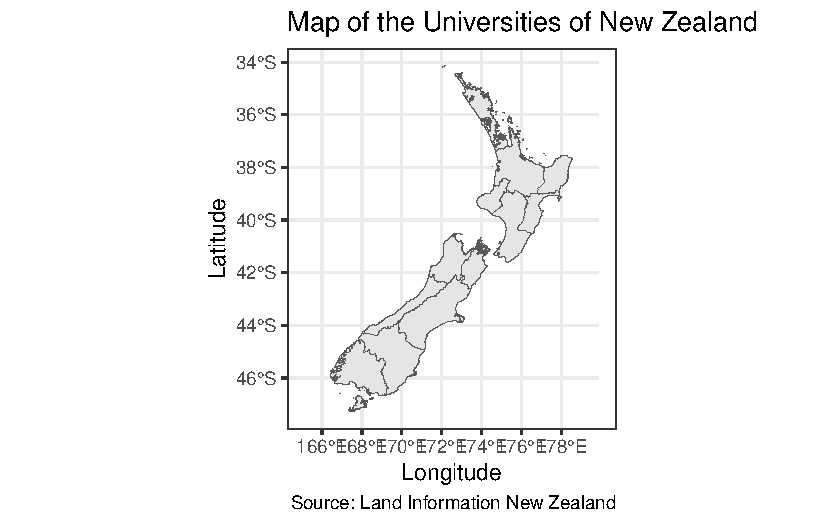
\includegraphics{Introduction-to-mapping_files/figure-pdf/making tighter map-2.pdf}

}

\end{figure}

\begin{Shaded}
\begin{Highlighting}[]
\CommentTok{\#|label: Add the unis}
\CommentTok{\# Add the Universities {-}{-}{-}{-}{-}{-}{-}{-}{-}{-}{-}{-}{-}{-}{-}{-}{-}{-}{-}{-}{-}{-}{-}{-}{-}{-}{-}{-}{-}{-}{-}{-}{-}{-}{-}{-}{-}{-}{-}{-}{-}{-}{-}{-}{-}{-}{-}{-}{-}{-}{-}{-}}
\DocumentationTok{\#\# we move the data for the map to the geom\_sf and the data for the labels to the geom\_label}
\FunctionTok{library}\NormalTok{(ggrepel)}
\FunctionTok{ggplot}\NormalTok{() }\SpecialCharTok{+}
  \FunctionTok{geom\_sf}\NormalTok{(}\AttributeTok{data =}\NormalTok{ trimmed) }\SpecialCharTok{+}
  \FunctionTok{coord\_sf}\NormalTok{(}\AttributeTok{xlim =} \FunctionTok{c}\NormalTok{(}\DecValTok{165}\NormalTok{, }\DecValTok{180}\NormalTok{)) }\SpecialCharTok{+}
  \FunctionTok{geom\_label\_repel}\NormalTok{(}\AttributeTok{data =}\NormalTok{ NZUs, }\FunctionTok{aes}\NormalTok{(}\AttributeTok{x =}\NormalTok{ lng, }\AttributeTok{y =}\NormalTok{ lat, }\AttributeTok{label =}\NormalTok{ Universities)) }\SpecialCharTok{+}
  \FunctionTok{theme\_economist}\NormalTok{() }\SpecialCharTok{+}
  \FunctionTok{ggtitle}\NormalTok{(}\StringTok{"Map of the Universities of New Zealand"}\NormalTok{) }\SpecialCharTok{+}
  \FunctionTok{labs}\NormalTok{(}\AttributeTok{x =} \StringTok{"Longitude"}\NormalTok{, }
       \AttributeTok{y =} \StringTok{"Latitude"}\NormalTok{, }
       \AttributeTok{caption =} \StringTok{"Source: University coordinates from google maps"}\NormalTok{) }
\end{Highlighting}
\end{Shaded}

\begin{figure}[H]

{\centering 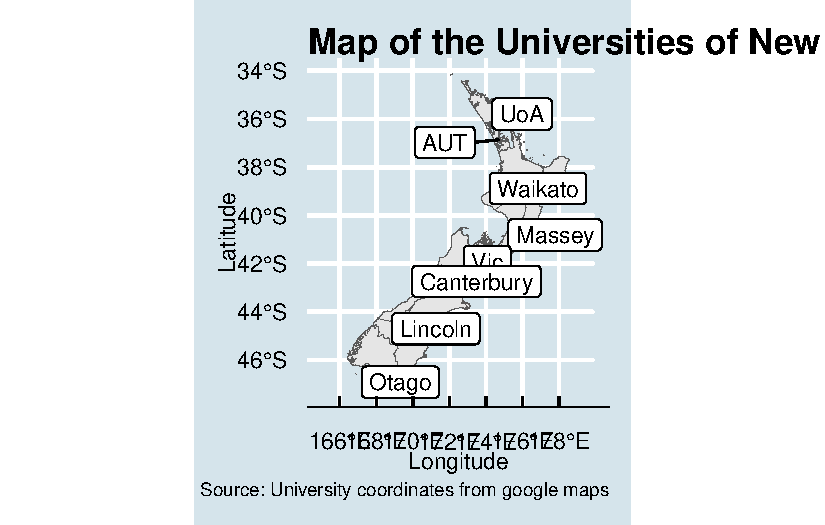
\includegraphics{Introduction-to-mapping_files/figure-pdf/unnamed-chunk-21-1.pdf}

}

\end{figure}



\end{document}
